\section{Finite Volume Method for the Shallow Water Equations}
In this section we will describe the Finite Volume Method (FVM) for solving the shallow water equations (SWE).
In the FVM, we discretize the domain into finite control volumes
\begin{align*}
    V_i = [x_{i-1/2}, x_{i+1/2}] \times [t_n, t_{n+1}],
\end{align*}
where $\Delta x = x_{i+1/2} - x_{i-1/2}$ is the length of the cell and $\Delta t = t_{n+1} - t_n$ is the time step.




For a finite volume $V_i^n$, we average the integral form~\eqref{eq:integral_form_1D_final} over the volume to get the explicit conservative formula:
\begin{align}\label{eq:explicit_conservative_1D_SWE}
    \mathbf{U}_i^{n+1} = \mathbf{U}_i^n - \frac{\Delta t}{\Delta x} \left( \mathbf{F}_{i+1/2}^n - \mathbf{F}_{i-1/2}^n \right) + \Delta t \mathbf{S}_i,
\end{align}
where $\mathbf{U}_i^n$ approximates the cell average over the $i$-th cell at time $t_n$:
\begin{align}
    \mathbf{U}_i^n \approx \frac{1}{\Delta x} \int_{x_{i-1/2}}^{x_{i+1/2}} \mathbf{U}(x,t_n) \text{ d}x,
\end{align}
where $\Delta x = x_{i+1/2} - x_{i-1/2}$ is the length of the cell.
The value $\mathbf{F}_{i-1/2}^n$ approximates the average flux along the line $x = x_{i-1/2}$ at time $t_n$:
\begin{align*}
    \mathbf{F}_{i-1/2}^n \approx \frac{1}{\Delta t} \int_{t_n}^{t_{n+1}} \mathbf{F}(\mathbf{U}(x_{i-1/2},t)) \text{ d}t,
\end{align*}
and the source term $\mathbf{S}_i$ approximates the average source term over the $i$-th cell at time $t_n$:
\begin{align*}
    \mathbf{S}_i &= \frac{1}{\Delta t \Delta x} \int_{t_n}^{t_{n+1}} \int_{x_{i-1/2}}^{x_{i+1/2}} \mathbf{S}(x,t) \text{ d}x\text{d}t.
\end{align*}


In the FVM, we discretize the domain into cells or control volumes.
Then we solve the local Riemann problem at the cell interface to obtain the fluxes.
Using the computed fluxes, we update the solution in each cell.
This way, the FVM allows for discountinuous solutions, as we solve the Riemann problem at the cell interfaces.
Therefore it is well suited for hyperbolic conservation laws, such as the shallow water equations.


\subsection{Finite Volume Methods for the 1D SWE}
We begin by considering finite volume methods for the SWE in one space dimension.
Recall that the homogeneous 1D SWE are given by
\begin{align*}
    h_t + {(hu)}_x &= 0, \\
    {(hu)}_t + {\left(hu^2 + \frac{1}{2}gh^2\right)}_x &= 0.
\end{align*}

A finite volume method for the 1D SWW is based on dividing the spatial domain into a set of intervals, also called grid cells.
The grid is illustrated in Figure~\ref{fig:FVM_1D_grid}.
\begin{figure}[H]
    \centering
    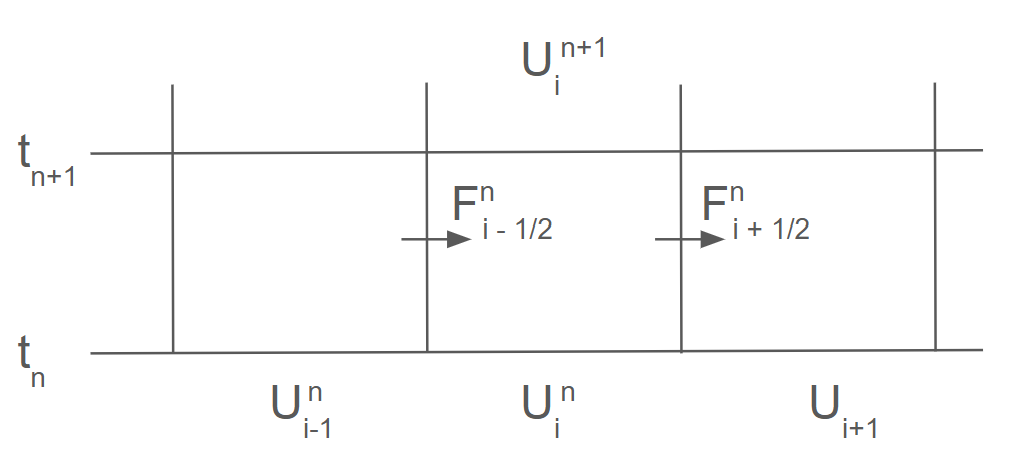
\includegraphics[width=0.5\textwidth]{C:/Users/Matteo/Shallow-Water-Equations/figs/FVM_1D_grid.png}
    \caption{Illustration of the grid for the 1D SWE.}\label{fig:FVM_1D_grid}
\end{figure}



This approach~\eqref{eq:explicit_conservative_1D_SWE} is called a finite volume scheme, since it is based on the integral conservation over finite volumes.
Note that the main difference between the FVM and the FDM is that the FVM is based on the integral conservation over finite volumes, whereas the FDM is based on the differential conservation over finite differences.
The main idea in the FVM is to define the numerical flux $\mathbf{F}_{i+1/2}^n$ at the cell inerface as a function of the cell averages $\mathbf{U}_i^n$ and $\mathbf{U}_{i+1}^n$.
Since only the cell-averages solution is known.
This also means that the FVM does not provide pointwise values of the solution, i.e., $\mathbf{U}(x,t)$, but only the cell-averages $\mathbf{U}_i^n$ over the control volume.

Throughout this report, we will assume a uniform grid for simplicity.
A key problem is to determine good numerical flux functions, that based on the cell averages, which is our only data, approximates the fluxes reasonable well. 



\subsection{Finite Volume Method for the 1D SWE with source term}
Consider the inhomoegeneous non-linear system
\begin{align*}
    \mathbf{U}_t + \mathbf{F(U)}_x = \mathbf{S(U)},
\end{align*} 
where $\mathbf{S(U)}$ is a vector of sources. 



\subsection{Finite Volume Method for the 2D SWE}
Follows the methods outlined in~\cite{Toro2009-Riemann}.
Consider a time-dependent two dimensional system of conservation laws
\begin{align}\label{eq:2D_SWE}
    \mathbf{U}_t + \mathbf{F(U)}_x + \mathbf{G(U)}_y = 0.
\end{align}
A numerical explicit finite volume scheme to solve~\eqref{eq:2D_SWE} is given by
\begin{align}
    \mathbf{U}_{i,j}^{n+1} = \mathbf{U}_{i,j}^n + \frac{\Delta t}{\Delta x}(\mathbf{F}_{i-1/2,j} - \mathbf{F}_{i+1/2,j}) + \frac{\Delta t}{\Delta y}(\mathbf{G}_{i,j-1/2} - \mathbf{G}_{i,j+1/2}).
\end{align}
This is the unsplit finite volume method, meaning that, in a single step, the cell average $\mathbf{U}_{i,j}^n+$ is updated using the fluxes from all intercell boundaries.

